\documentclass{article}
\usepackage[utf8]{inputenc}
\usepackage[T1]{fontenc}
\usepackage{booktabs}
\usepackage{xcolor}
\usepackage{fontawesome5}
\usepackage{geometry}
\usepackage{array}
\usepackage{helvet}
\usepackage{titlesec}
\usepackage{parskip}
\usepackage{mdframed}
\usepackage{hyperref}
\usepackage{ragged2e}
\usepackage{graphicx}
\usepackage{ccicons}
\usepackage{fancyhdr}
\usepackage{lmodern}
\usepackage[export]{adjustbox}

% Meta-Informationen für den PDF-Export
\hypersetup{
    pdftitle={Teilnehmerliste \& Datenschutz in Moodle},
    pdfauthor={Christian-Maximilian Steier},
    pdfsubject={Datenschutzkonformer Umgang mit der Teilnehmerliste in Moodle},
    pdfkeywords={Moodle, Teilnehmerliste, Datenschutz, DSGVO, viewparticipants, Christian-Maximilian Steier},
    colorlinks=true,
    linkcolor=customred,
    urlcolor=customred,
    pdfborderstyle={/S/U/W 1}
}

\renewcommand{\familydefault}{\sfdefault}

% Keine Worttrennung
\tolerance=1
\emergencystretch=\maxdimen
\hyphenpenalty=10000
\hbadness=10000
\raggedright

\geometry{a4paper, margin=2.5cm}
\definecolor{customred}{RGB}{230, 0, 40}
\definecolor{lightred}{RGB}{255, 235, 238}
\definecolor{lightblue}{RGB}{235, 245, 255}
\definecolor{lightgray}{RGB}{245, 245, 245}
\definecolor{ccboxborder}{RGB}{200, 200, 200}
\definecolor{ccboxbg}{RGB}{245, 245, 245}

% Titelgestaltung
\titleformat{\section}
  {\normalfont\Large\bfseries\color{customred}}
  {}{0em}{}[\vspace{-0.5em}\rule{\textwidth}{0.5pt}]

% Fußzeile
\pagestyle{fancy}
\fancyhf{}
\renewcommand{\headrulewidth}{0pt}
\fancyfoot[C]{
\ccby{}\quad Dieses Dokument wurde erstellt von \textbf{ZWEK} der Hochschule Düsseldorf und steht unter der Lizenz \textbf{CC BY 4.0}.  
Weitere Informationen: \url{https://creativecommons.org/licenses/by/4.0/}\\
\textsf{\small{Stand: August 2025 \textbullet{} Moodle Version 4.5}}}
\fancyfoot[R]{\textsf{\thepage}}

% Gemeinsame Breite
\newlength{\commonwidth}
\setlength{\commonwidth}{16cm}

\begin{document}

% Titel
\begin{center}
\textbf{\textcolor{customred}{\LARGE Teilnehmerliste \faUsers{} \& Datenschutz \faUserShield}}
\end{center}

\vspace{0.5cm}

% Anwendungsfall Box
\begin{center}
\begin{minipage}{\commonwidth}
\begin{mdframed}[backgroundcolor=lightgray, linewidth=0pt, roundcorner=5pt]
\textbf{Anwendungsfall:}

Sie möchten die Teilnehmerliste in Ihrem Moodle-Kurs aus Datenschutzgründen einschränken -- z.\,B. bei Prüfungskursen, Kursen mit sensiblen Inhalten oder um den Schutz personenbezogener Daten gemäß DSGVO zu gewährleisten.

\vspace{0.3cm}

\textbf{Szenarien:}
\begin{itemize}
  \item \textbf{Klausurkurse:} Teilnehmende sollen keine Möglichkeit haben, während der Klausur miteinander zu kommunizieren.
  \item \textbf{Sensible Lehrinhalte:} Teilnahme an bestimmten Kursen soll nicht für alle sichtbar sein (z.\,B. Psychologie, Medizin, Recht).
  \item \textbf{Datenschutz:} Namen, E-Mail-Adressen und Profile sollen nicht grundsätzlich für alle Kursteilnehmenden einsehbar sein.
\end{itemize}
\end{mdframed}
\end{minipage}
\end{center}

\vspace{0.8cm}

% Lösungsansätze im Überblick
\textbf{Lösungsansätze im Überblick:}

Es gibt zwei grundlegende Möglichkeiten, die Sichtbarkeit der Teilnehmerliste in Moodle zu steuern:

\begin{enumerate}
  \item \textbf{Berechtigung auf Kursebene ändern} (empfohlen) -- Individuelle Anpassung pro Kurs
  \item \textbf{Berechtigung auf Kategorie-Ebene ändern} -- Änderung für alle Kurse einer Kategorie
\end{enumerate}

\vspace{0.6cm}

\renewcommand{\arraystretch}{1.4}
\setlength{\tabcolsep}{8pt}

% Vergleichstabelle
\begin{center}
\begin{minipage}{\commonwidth}
\begin{tabular}{>{\bfseries\raggedright\arraybackslash}p{3.5cm}>{\raggedright\arraybackslash}p{6cm}>{\raggedright\arraybackslash}p{6cm}}
\toprule
\textcolor{customred}{\textbf{}} 
& \textbf{Kursebene \faLayerGroup} 
& \textbf{Kategorie-Ebene \faFolder} \\
\midrule
Reichweite 
       & \faMapMarker~Nur für den ausgewählten Kurs 
       & \faFolder~Für alle Kurse einer Kategorie \\
\midrule
Zugriff 
       & \faCogs~Kurs $\rightarrow$ Teilnehmer $\rightarrow$ Berechtigungen 
       & \faCogs~Administration $\rightarrow$ Kurse $\rightarrow$ Kategorie $\rightarrow$ Rechte \\
\midrule
Flexibilität 
       & \faSlidersH~Kurse einzeln konfigurierbar 
       & \faLock~Einheitlich für alle Kurse einer Kategorie \\
\midrule
Empfehlung 
       & \faCheckCircle~\textcolor{customred}{Empfohlen} für gezielte Einschränkung 
       & \faExclamationTriangle~Nur bei einheitlichem Bedarf \\
\midrule
Datenschutz 
       & \faUserShield~Feingranulare Steuerung 
       & \faUserShield~Grober, aber einheitlich \\
\bottomrule
\end{tabular}
\end{minipage}
\end{center}

\vspace{0.7cm}

% Anleitung Box: Kursebene
\begin{center}
\begin{minipage}{\commonwidth}
\fcolorbox{customred!30}{lightblue!30}{%
    \begin{minipage}{\dimexpr\commonwidth-2\fboxsep-2\fboxrule}
    \raggedright
    \textbf{\textcolor{customred}{Anleitung: Berechtigung auf Kursebene ändern}}
    
    \vspace{0.3cm}
    
    \begin{enumerate}
      \item Öffnen Sie den gewünschten Kurs und klicken Sie auf \textbf{Teilnehmer/innen} in der Navigation.
      \item Wählen Sie im Dropdown-Menü \textbf{Rechte} aus.
      \item Suchen Sie im Filter \texttt{viewparticipants}.
      \item Setzen Sie die Rolle \textbf{Studierende} auf \textbf{Verbieten}.
      \item Bestätigen Sie mit \textbf{Änderungen speichern}.
    \end{enumerate}
    
    \vspace{0.3cm}
    
    \textbf{Wichtig:} Verwenden Sie \textbf{Verbieten} statt \textbf{Nicht gesetzt}, um die Einschränkung sicher durchzusetzen. ``Verbieten'' überschreibt alle anderen Berechtigungen und kann nicht durch übergeordnete Rollen aufgehoben werden.
    \end{minipage}%
}
\end{minipage}
\end{center}

\vspace{0.8cm}

% Schritt 1
\noindent\textbf{Schritt 1: Teilnehmerbereich öffnen}

Öffnen Sie den gewünschten Kurs und klicken Sie auf \textbf{Teilnehmer/innen} in der Navigation.

\begin{center}
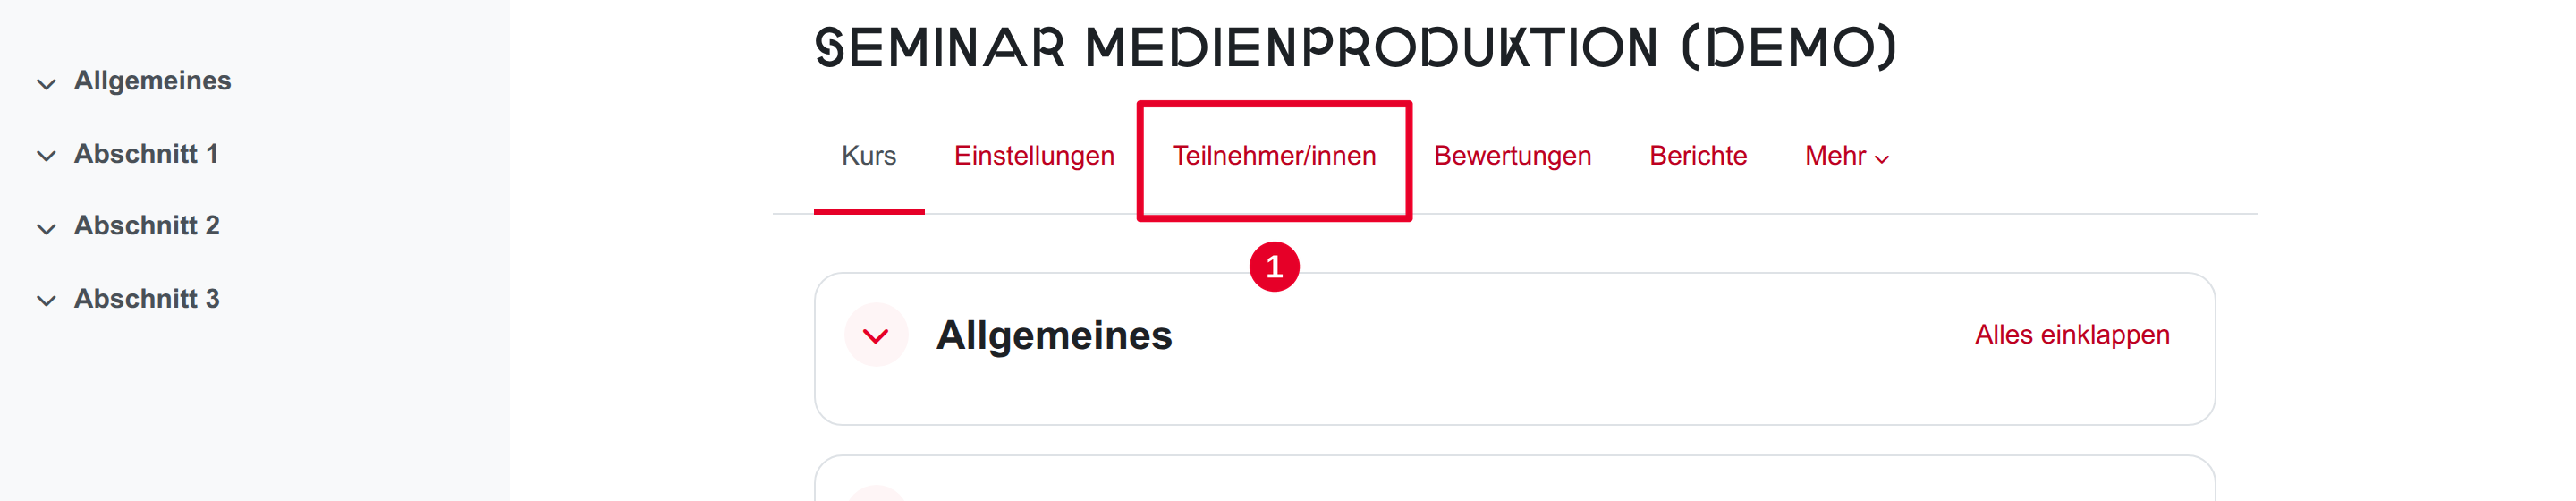
\includegraphics[width=0.95\commonwidth]{Bilder/Bild1.png}\\[0.3cm]
\small\textbf{Abb. 1:} Kursnavigation -- \emph{Teilnehmer/innen} anklicken
\end{center}

\vspace{0.7cm}

% Schritt 2
\noindent\textbf{Schritt 2: Berechtigungen öffnen}

Klicken Sie auf das Dropdown-Menü \textbf{Eingeschriebene Nutzer/innen} und wählen Sie \textbf{Rechte} aus.

\begin{center}
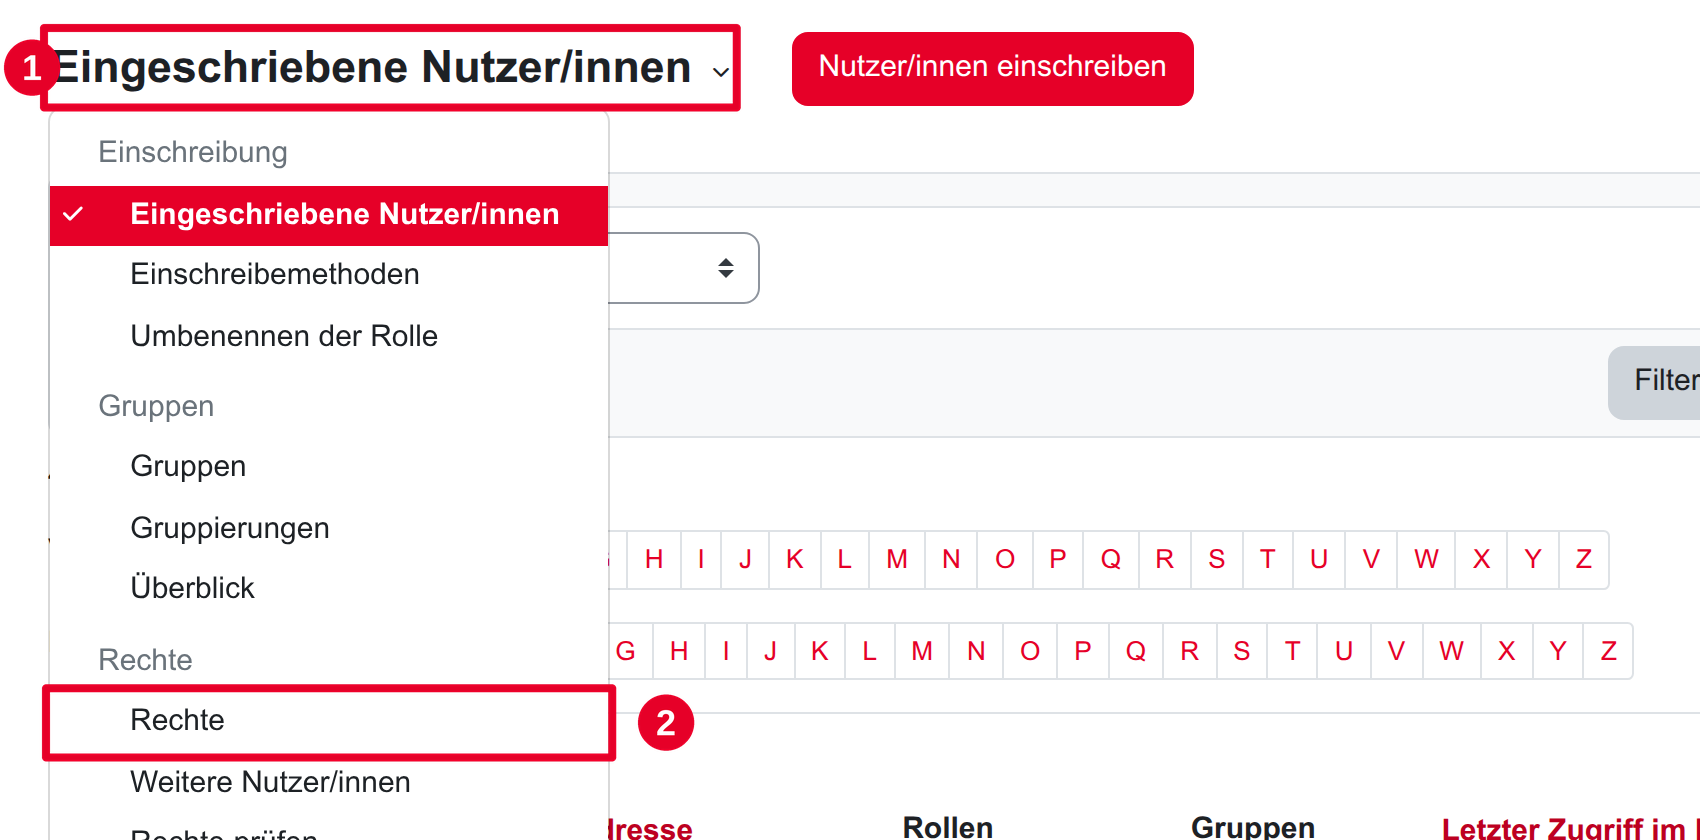
\includegraphics[width=0.95\commonwidth]{Bilder/Bild2.png}\\[0.3cm]
\small\textbf{Abb. 2:} Dropdown-Menü $\rightarrow$ \emph{Rechte} wählen
\end{center}

\vspace{0.7cm}

% Schritt 3
\noindent\textbf{Schritt 3: \texttt{moodle/course:viewparticipants} suchen}

Suchen Sie in der Übersichtstabelle die Zeile mit der Capability \texttt{moodle/course:viewparticipants}.

\begin{center}
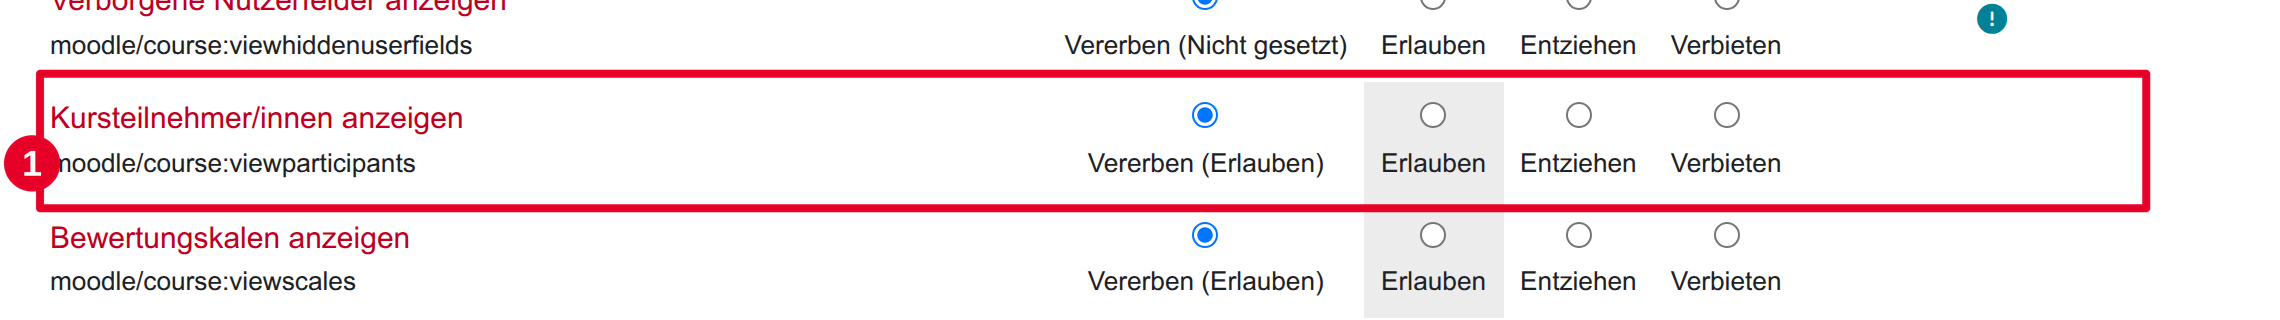
\includegraphics[width=0.95\commonwidth]{Bilder/Bild3.png}\\[0.3cm]
\small\textbf{Abb. 3:} Zeile \texttt{moodle/course:viewparticipants} finden
\end{center}

\vspace{0.7cm}

% Schritt 4
\noindent\textbf{Schritt 4: Studierende von der Teilnehmerliste ausschließen -- \textcolor{customred}{WICHTIGSTER SCHRITT}}

Setzen Sie die Berechtigung für die Rolle \textbf{Studierende} auf \textbf{Verbieten}.

\begin{center}
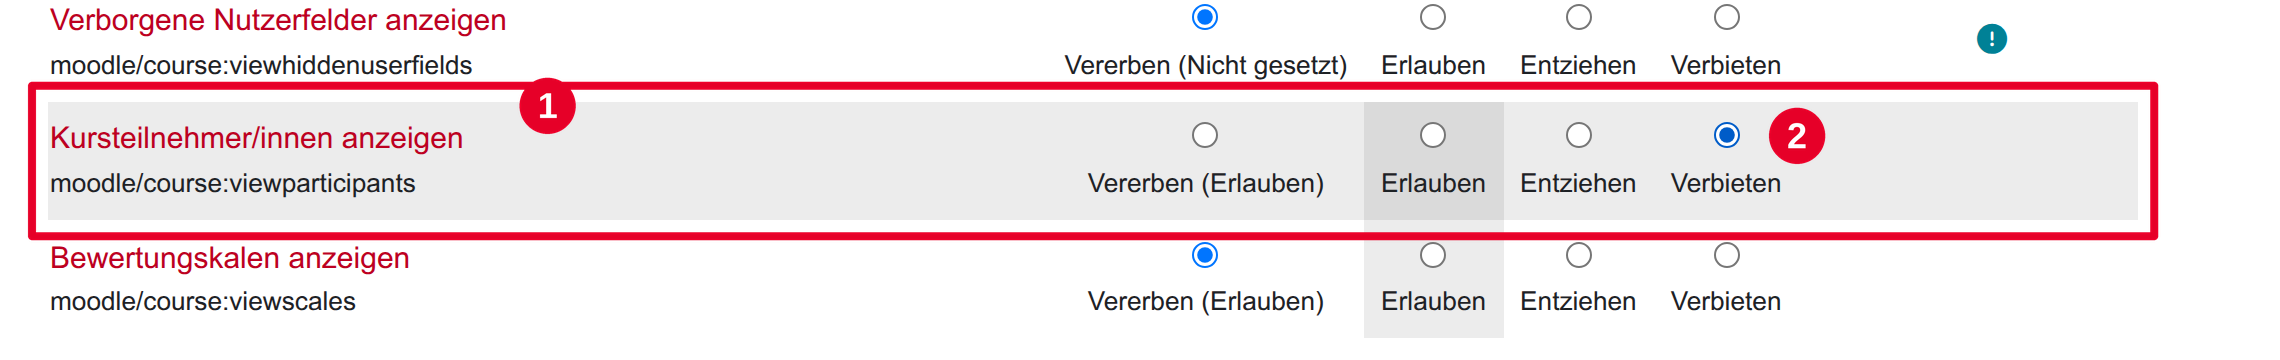
\includegraphics[width=0.95\commonwidth]{Bilder/Bild4.png}\\[0.3cm]
\small\textbf{Abb. 4:} \textbf{Wichtigste Einstellung:} Für die Rolle \emph{Studierende} die Berechtigung auf \textbf{Verbieten} setzen
\end{center}

\vspace{0.7cm}

% Schritt 5
\noindent\textbf{Schritt 5: Änderungen speichern}

Bestätigen Sie die Änderung mit dem Button \textbf{Änderungen speichern}.

\vspace{0.7cm}

% Auswirkungen
\section{Auswirkungen und mögliche Nebeneffekte}

\textbf{Direkte Auswirkung}

Die Teilnehmerliste ist für Studierende nicht mehr sichtbar.

\vspace{0.3cm}

\textbf{Mögliche Nebeneffekte}

\begin{itemize}
  \item Die Suche nach anderen Kursteilnehmenden kann eingeschränkt sein.
  \item Die @mention-Funktion in Foren kann beeinträchtigt sein.
  \item Bei Gruppenarbeiten kann die Sichtbarkeit von Gruppenmitgliedern eingeschränkt werden.
\end{itemize}

\vspace{0.7cm}

% Literatur und Links Box
\begin{center}
\begin{minipage}{\commonwidth}
\begin{mdframed}[
    backgroundcolor=lightgray, 
    linewidth=0pt, 
    roundcorner=5pt,
    innerleftmargin=1em,
    innerrightmargin=1em,
    innertopmargin=0.7em,
    innerbottommargin=0.7em
]
\raggedright
\textbf{\textcolor{customred}{Literatur \& Links zum Thema}}
\vspace{0.2cm}

\begin{itemize}
\item \textbf{Offizielle Moodle-Dokumentation:}
\vspace{0.2cm}
  \begin{itemize}
  \item Teilnehmer/innen: \url{https://docs.moodle.org/de/Teilnehmer/innen}
  \item Capability viewparticipants: \url{https://docs.moodle.org/en/Capabilities/moodle/course:viewparticipants}
  \end{itemize}
\vspace{0.5cm}
\end{itemize}
\end{mdframed}
\end{minipage}
\end{center}

\end{document}
